\section{Evaluation}
\label{sec:results}

We present an evaluation study of our implementation, report contract
profiles of benchmark programs, and illustrate the performance benefits of
fine-grained consistency classification on operations and transactions. We
also evaluate the impact of the summarization. We have implemented the
following applications, which includes individual RDTs as well as larger
applications composed of several RDTs:

\begin{itemize}
\setlength{\itemsep}{2pt}
\item \textbf{LWW register}: A last-write-wins register that provides read
  and write operations. Each write is associated with a timestamp, which is
  used to resolve conflicting concurrent writes -- a newer write always
  wins.

\item \textbf{DynamoDB register}: An integer register that allows eventual
  and strong puts and gets, conditional puts, increment and decrement
  operations.

\item \textbf{Bank account}: Our running example, with savings and checking
  accounts.

\item \textbf{Shopping list}: A collaborative shopping list that allows
  adding and deleting items.

\item \textbf{Online store}: An online store with shopping cart
  functionality and dynamically changing item prices.  The checkout process
  verifies that the customer only pays the accepted price.

\item \textbf{RUBiS}: An ebay-like auction site~\cite{RUBiS}. The
  application allows users to browse items, bid for items on sale, and pay
  for items from a wallet modelled after a bank account.

\item \textbf{Microblog}: A twitter-like microblogging site, modelled after
  Twissandra~\cite{Twissandra}. The application allows adding new users,
  adding and replying to tweets, following, unfollowing and blocking users,
  and fetching a user's timeline, userline, followers and following.
\end{itemize}

\begin{table}
\setlength{\tabcolsep}{4pt}
{\sffamily \small
\begin{center}
\begin{tabular} {|l|r|r|r|r|r|r|r|r|}
\hline
{\bf Benchmark} & {\bf LOC} & {\bf \#T} & {\bf EC} & {\bf CC} & {\bf SC} & {\bf RC} & {\bf MAV} & {\bf RR} \\
\hline
{LWW Reg} & 108 & 1 & 2 & 2 & 2 & 0 & 0 & 0 \\
{DynamoDB} & 126 & 1 & 3 & 1 & 2 & 0 & 0 & 0 \\
{Bank Account} & 155 & 1 & 1 & 1 & 1 & 1 & 0 & 1 \\
{Shopping List} & 140 & 1 & 2 & 1 & 1 & 0 & 0 & 0 \\
{Online store} & 340 & 4 & 9 & 1 & 0 & 2 & 0 & 1 \\
{RUBiS} & 640 & 6 & 14 & 2 & 1 & 4 & 2 & 0 \\
{Microblog} & 659 & 5 & 13 & 6 & 1 & 6 & 3 & 1 \\
\hline
\end{tabular}
\end{center} }
\caption{The distribution of classified contracts. \#T refers to the number of
tables in the application. The columns 4-6 (7-9) represent operations
(transactions) assigned to this consistency (isolation) level.}
\label{tab:ctrts}
\end{table}

The distribution of contracts in these applications is given in
Table~\ref{tab:ctrts}. We see that majority of the operations and
transactions are classified as eventually consistent and RC,
respectively. Operation contracts are used to enforce integrity and
visibility constraints on individual fields in the tables. Transactions are
mainly used to consistently modify and access related fields across
tables. In \name, the contract classification process is completely
performed at compile time and has no overheads at runtime. The proof
obligations associated with contract classification is discharged through
the Z3 SMT Solver. Across our benchmarks, classifying a contract took 11.5
milliseconds on average.

For our performance evaluation, we deploy \name applications in
\emph{clusters}, where each cluster is composed of five fully replicated
Cassandra replicas within the same datacenter. We instantiate one shim layer
node co-located on the same VM as a Cassandra replica. Clients are
instantiated within the same data center as the store, and run
transactions. We deploy each node in the cluster on \cf{c3.4xlarge} Amazon
EC2 instances.  Our shim layer nodes are multi-threaded, and we allocate 8
CPUs (out of 16 available) for each shim layer node. The clients also run on
\cf{c2.4xlarge} instances. We call this a \cf{1DC} configuration. For our
geo-distributed experiments (\cf{2DC}), we instantiate 2 clusters, each with
five nodes, and place the clusters on US-east (Virginia) and US-west
(Oregon) locations. The average inter-region latency was 85ms.

\begin{figure*}
  \centering
  \subfigure[Bank account]{\label{grf:BA-tp-vs-lat}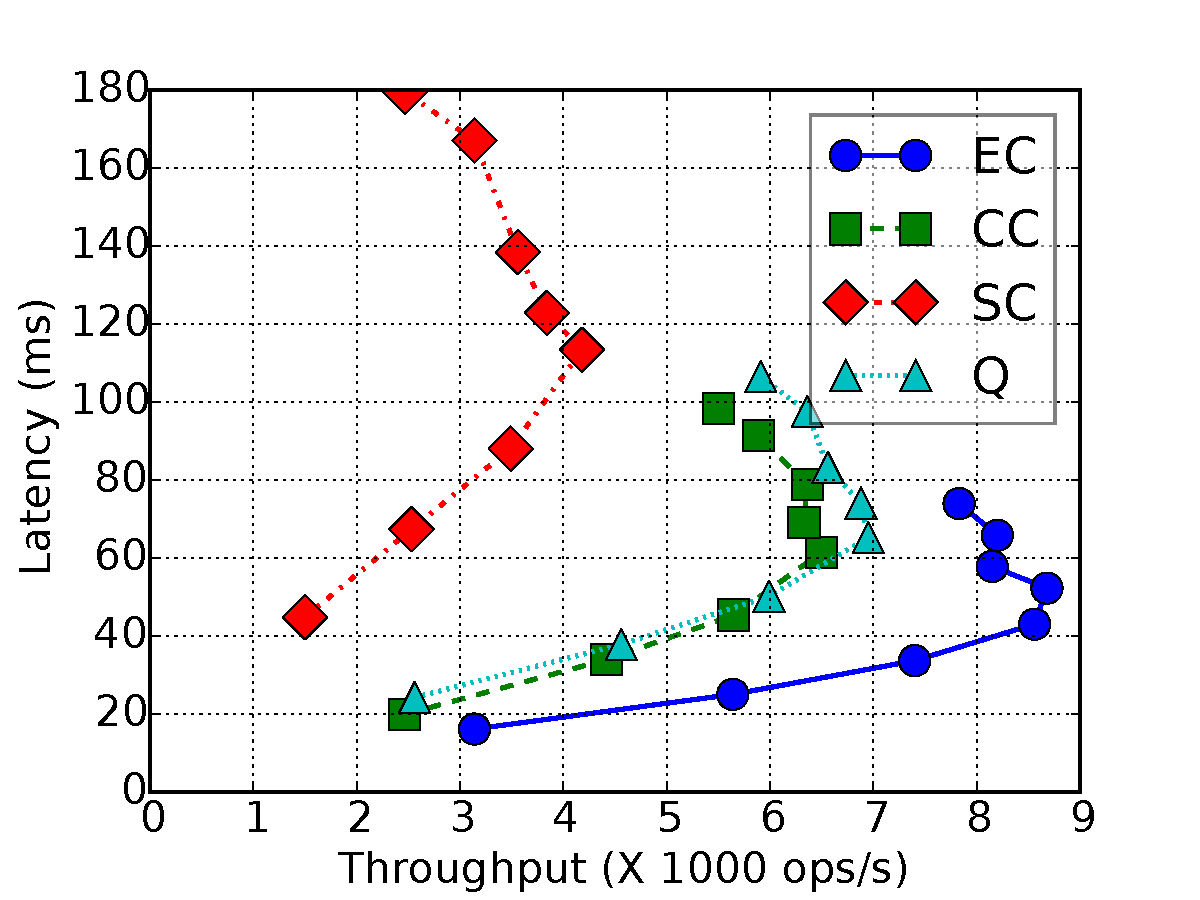
\includegraphics[width=0.24\textwidth]{graphs/BA-tp-vs-lat.pdf}}
  \subfigure[LWW transactions]{\label{grf:LWW-txn}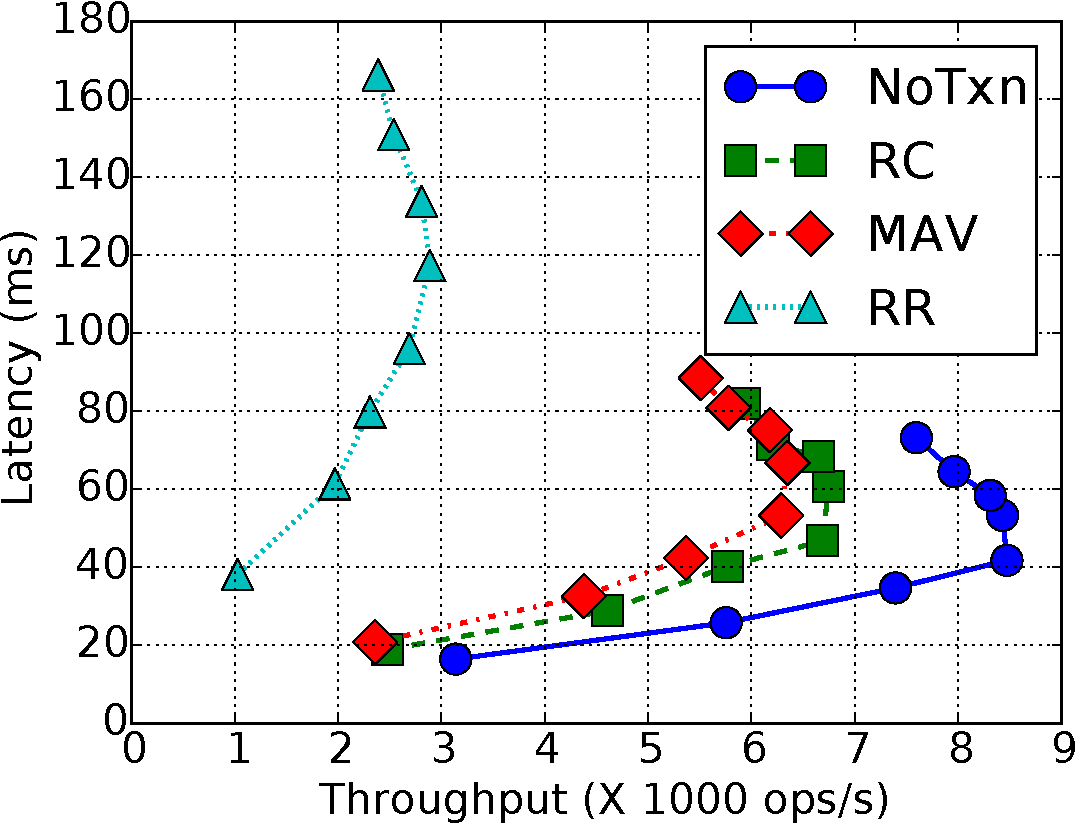
\includegraphics[width=0.24\textwidth]{graphs/LWW-txn.pdf}}
  \subfigure[RUBiS bidding mix]{\label{grf:rubis}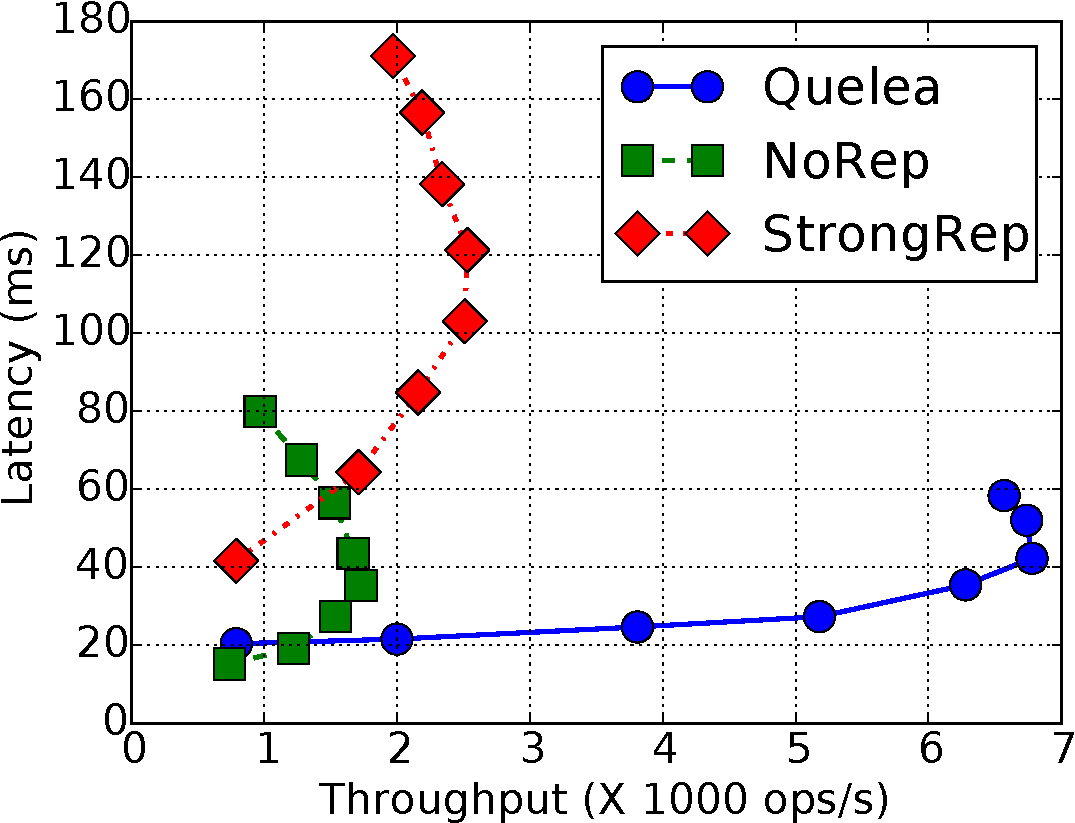
\includegraphics[width=0.24\textwidth]{graphs/Rubis.pdf}}
  \subfigure[Impact of summarization]{\label{grf:summarization}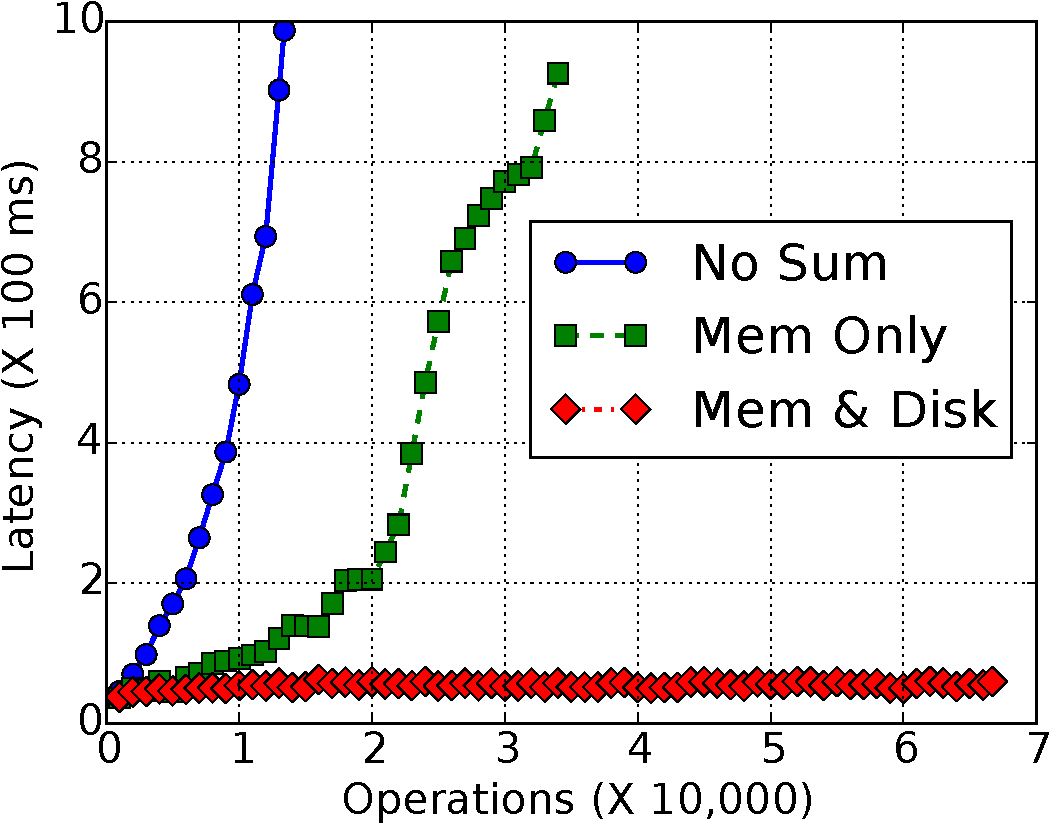
\includegraphics[width=0.235\textwidth]{graphs/summarization.pdf}}
	\caption{Quelea Performance.}
  \label{grf:LWW_perf}
\end{figure*}

Figure~\ref{grf:BA-tp-vs-lat} shows throughput vs. latency of operations
in the bank account example as we increase the number of clients in a \cf{1DC}
configuration. Our client workload was generated using the YCSB
benchmark~\cite{YCSB}. The benchmark uniformly chooses from 100,000 keys, where
the operation spread was 25\% withdraw, 25\% deposit and 50\% getBalance, which
corresponds to the default 50:50 read:write mix in YCSB. We increased the
number of clients from 128 to 1024, and each experiment ran for 180 seconds.

The lines marked EC and CC correspond to all operations (including
\cf{withdraw}) being assigned EC and CC consistency levels. These levels
compromise correctness as \cf{withdraw} has to be an SC operation. The SC
line corresponds to a configuration where all operations are strongly
consistent; this ensures application correctness, at the cost of
performance. \name corresponds to our implementation, which classifies
operations based on their contract specifications.  Both \name and SC ensure
correctness. With 512 clients, the \name implementation was within 41\% of
the latency and 18\% of the throughput of EC, whereas SC operations had
162\% higher latency and 52\% lower throughput than EC operations. Observe
that there is a point in each case after which the latency increases while
the throughput decreases; these points correspond to client request
saturation points in the data store.

In a \cf{2DC} configuration (not shown here), the average latency of SC
operations with 512 clients increased by 9.4$\times$ due to the cost of
geo-distributed coordination, whereas \name operations were only 2.2$\times$
slower, mainly due to the increased cost of \cf{withdraw}
operations. Importantly, the latency of \cf{getBalance} and \cf{deposit}
remained almost the same, illustrating the benefit of fine-grained
contract classification.

We compare the performance of different transaction isolation level choices
in Figure~\ref{grf:LWW-txn} using the LWW register. The numbers were
obtained under a 1DC configuration. The YCSB workload was modified to issue
10 operations per transaction, with a default 50:50 read:write mix. Each
operation is assumed to be eventual consistent. \cf{NoTxn} corresponds to a
configuration that does not use transactions. Compared to this, RC is only
12\% shower in terms of latency with 512 clients, whereas RR is 2.3X
slower. The difference between RC and \cf{NoTxn} is due to the meta-data
overhead of recording transaction information in the object state. For RR
transactions, the cost of capturing and maintaining a snapshot is the
biggest source of overhead.

We also compared (not shown) the performance of EC LWW operations directly
against Cassandra, which uses last-writer-wins as the only convergence
semantics. While Cassandra provides no stronger-than-eventual consistency
properties, \name was within 30\%(20\%) of latency(throughput) of Cassandra
with 512 clients, supporting our thesis that programmers only have to incur
relatively low overhead for a more expressive programming model which
provides stronger provable consistency guarantees.

Figure~\ref{grf:rubis} compares the \name implementation of RUBiS in a
\cf{1DC} configuration against a single replica ({\sf NoRep}) and a strongly
replicated ({\sf StrongRep}) \cf{1DC} deployment. The benchmark uses the
default RUBiS bidding mix, which has 15\% read-write interactions, which is
representative of the auction workload.  Without replication, {\sf NoRep}
trivially provides strong consistency. However, this deployment does not
scale beyond 1750 operations per second. Strong replication offers better
throughput at the cost of greater latency due to inter-replica
coordination. The \name deployment offers the benefit of replication, while
only paying the cost of coordination when necessary.

Finally, we study the impact of summarization in
Figure~\ref{grf:summarization}. We use 128 clients and a single \name
replica, with all clients operating on the \emph{same} LWW register to
stress test the summarization mechanism. The shim layer cache (memory) is
summarized every 64 updates, while the updates in the backing store (disk)
are summarized every 4096 updates. Each point in the graph represents the
average latency of the previous 1000 operations. Each experiment is run for
one minute.  Without summarization, the average latency of operations
increases exponentially to almost one second, and only 13K operations were
performed in a minute. Since every operation has to reduce over the set of
all previous operations, operations take increasingly more time to complete
since they must contend with an ever growing set.  With summarization only
in memory, performance still degrades due to the cost of fetching all
previous updates from the backing store into the shim layer. Fetching the
latest updates is essential for SC operations. With summarization enabled on
both disk and memory, latency does not increase over time, and the
implementation realizes throughput of 67K operations/minute. 
